\chapter{Кинематика твердого тела. Поступательное движение.}
\begin{table}[h!]
    \vspace*{-2em}
    \begin{tabular}{C{.45}m{.5\textwidth}}
        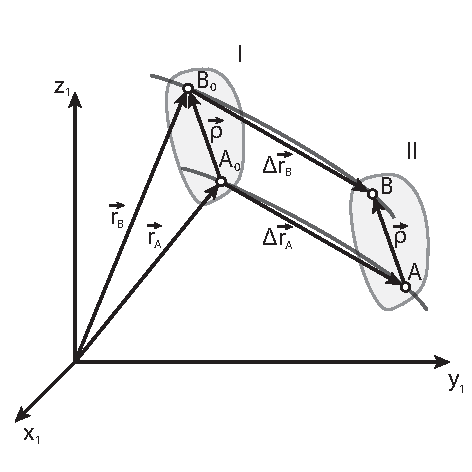
\includegraphics[width=.45\textwidth]{24_01} &
        Поступательным движением твердого тела называется такое движение, при
        котором любая прямая, проведенная в теле, остается во все время движения
        параллельной своему первоначальному положению.

        Пусть твердое тело движется поступательно относительно системы координат
        \( Ox_1y_1z_1 \), \( \vec{r}_A \) -- радиус-вектор точки \( A \),
        \( \vec{r}_B \) -- радиус-вектор точки \( B \), а \( \vec{\rho} \) --
        радиус-вектор, определяющий положение точки \( B \) в подвижной системе
        координат \( Axyz \), жестко связанной с телом.

        Так как тело абсолютно твердое и его движение поступательное, то вектор
        \( \vec{\rho} \) постоянный.
    \end{tabular}
    \vspace*{-1.5em}
\end{table}

Из рисунка следует: \( \vec{r}_B = \vec{r}_A + \vec{\rho} \). Пусть в момент
времени \( t \) тело занимало положение~I, а в момент времени \( t + \D t \) --
положение~II. Тогда \( \D\vec{r}_A \) и \( \D\vec{r}_B \) -- вектора перемещения
точек \( A \) и \( B \) за промежуток времени \( \D t \). Во время движения
вектор \( \vec{\rho} \) не изменяется, значит, отрезки \( A_0B_0 \) и \( AB \)
равны и параллельны и, следовательно, фигура \( A_0B_0BA \) -- параллелограмм.
Таким образом, \( \Delta\vec{r}_A = \Delta\vec{r}_B \), то есть при
поступательном движении абсолютно твердого тела перемещения всех его точек
геометрически равны между собой. Из рисунка и условия постоянства
\( \vec{\rho} \) также следует, что траектории точек тела, движущегося
поступательно, одинаковы и получаются друг из друга параллельным смещением.

Продифференцировав выражение для \( \vec{r}_B \) по времени, получим:
\[
    \der{\vec{r}_B}{t} = \der{\vec{r}_A}{t} + \der{\vec{\rho}}{t} =
    \der{\vec{r}_A}{t} \quad \text{ или } \quad \vec{v}_A = \vec{v}_B,
\]
то есть при поступательном движении твердого тела скорости всех его точек в
каждый момент времени равны между собой.

Дифференцируя полученное соотношение по времени, получим:
\[
    \der{\vec{v}_a}{t} = \der{\vec{v}_B}{t} \quad \text{ или } \quad
    \vec{a}_A = \vec{a}_B,
\]
то есть ускорения всех точек тела в каждый момент времени равны между собой.

Таким образом, при поступательном движении твердого тела все его точки движутся
одинаково, так как их перемещения, скорости и ускорения геометрически равны.

Иными словами, при поступательном движении абсолютно твердое тело можно заменить
материальной точкой и описывать движение этой точки вместо описания движения
множества точек твердого тела.

\newpage
